\documentclass[Main]{subfiles}
\begin{document}

\chapter{}
This chapter will cover the fundamentals in data distribution service (DDS), explaining the concept of middleware and DDS for real-time systems.
\section{Middleware}
In distributed systems, where multiple independent computers are connected on a network due to collaborating in achieving the same goal. These computers can be placed with different geographical locations and have different operating systems (OS) \cite[p. 2]{Tanenbaum}.
\\ To make the development of a distributed system easier the developers can use middleware, which is software between the application and the physical layers on the computer. The middleware contributes to the development as it hides the problems that can occur due to different software, hardware and OS's from each application \cite[p. 3]{Tanenbaum}.

\begin{figure}[hbtp]
\centering
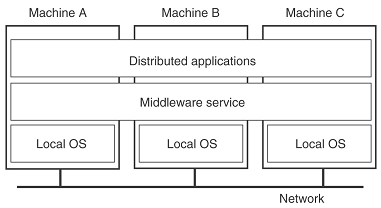
\includegraphics[scale=1]{Figure/Middleware.png}
\caption{A distributed system with middleware \cite[p. 3]{Tanenbaum}}
\label{Fig:Middleware}
\end{figure}

Each application is offered the same interface through the middleware layer which extends over multiple machines \cite[p. 3]{Tanenbaum}. The middleware is a principle that makes it easier for developers to scale a distributed system, as the developer can focus on the interface to the middleware and not the layers beneath. This makes the environment homogeneous as the differences in network technology, hardware architecture, OS, programming languages and geographical locations etc. \cite{DDS-slides} \cite[p. 68]{Coulouris}.
\\
To support the different programming languages used in the applications the middleware contains the Interface Definition Language (IDL). It takes care of mapping the language into IDL-standard before passing the data to the wanted computer, where the middleware again maps the data into the application language \cite{RTI}.
\\
Therefore middleware is useful when developing large and complex distributed systems as it connects the different parts with a "pipe" that makes data-sharing and communication efficient \cite{DDS-slides} \cite[p. 68]{Coulouris}. Also it should be considered that the middleware-software should be installed on all the involved computers which can raise the CPU load. Depending on the type of hardware that is used the developers should choose a sufficient middleware \cite{DDS-slides}.
\\
\\
When choosing between middlewares it is important to know which standard the different middlewares are using. There is a lot of standards that the middleware can support, e.g. which network the middleware supports or if the middleware supports a medical standard for transferring images and data between devices in the medical industry \cite{DDS_slides}.\\
There are various implementations of the standards e.g. OpenDDS by Object Computing Inc. which is an open source implementation. Among the commercial implementations Real-Time Innovations (RTI) has developed a middleware called Connext.


\end{document} 